\documentclass[12pt]{article}
\usepackage{xepersian}
\settextfont{XB Niloofar}
\setlatintextfont{Times New Roman}
\setlength{\parskip}{1em}

\usepackage{amsmath}
\usepackage{xcolor}
\usepackage{titlesec}
\usepackage{graphicx}
\graphicspath{{figures/}}
\usepackage{subcaption}
\usepackage{multirow}
\usepackage{tikz}
\usetikzlibrary{positioning, arrows.meta, shapes.geometric, fit, calc}

\begin{document}
	
	% ---------- Title page ----------
	\begin{center}
		\Large \textbf{گزارش کار آزمایشگاه مدار منطقی} \\[0.5em]
		\textbf{آزمایش چهارم}
	\end{center}
	
	\vspace{2em}
	
	\begin{center}
		دانشجویان:\\
		امیرحسین قرقانی -- 404106225\\
		محمد رجایی -- 404105842
	\end{center}
	
	
	\newpage
	
	% ---------- Section 1 ----------
	\section{شرح و هدف آزمایش}
	
	هدف از این آزمایش، آشنایی با نحوه طراحی و ساخت مدارهای کنترل‌کننده (ماشین حالت) با استفاده از نمودار حالت (\lr{ASM Chart}) است. در این آزمایش، پیاده‌سازی دو مدار کنترل‌کننده برای سیستم های «تایمر ماشین لباسشویی» و «تلفن راه‌دور» در محیط شبیه‌سازی \lr{Proteus} بررسی خواهد شد که طی مراحل اصلی زیر انجام می‌شود:
	
	\begin{itemize}
		\item \textbf{طراحی ماشین حالت (\lr{FSM}) و رسم \lr{ASM Chart}:} تحلیل وضعیت‌های سیستم و طراحی منطق تغییر وضعیت سیستم بر اساس سیگنال‌های ورودی (مانند \lr{Start, Door, Valve} در لباسشویی یا \lr{Coin, Reset} در تلفن) و خروجی‌های مورد نیاز (مانند مراحل مختلف شست‌وشو یا وضعیت‌های تماس و هشدار).
		
		\item \textbf{طراحی بخش‌های شمارش و ذخیره‌سازی:} استفاده از شمارنده‌های \lr{BCD} با قابلیت شمارش بالا/پایین برای نگهداری مقادیر
		
		\item \textbf{پیاده‌سازی ماشین حالت:} ساخت ماشین حالت با استفاده از فلیپ‌فلاپ‌های نوع \lr{D} و گیت‌های منطقی پایه جهت مدیریت تغییرات حالت در سیکل های متوالی.
		
		\item \textbf{طراحی بخش زمان‌سنجی:} استفاده از تایمرهای سنکرون (مانند تراشه ۷۴۱۶۳) جهت مدیریت زمان‌بندی‌ها.
		
	\end{itemize}
	
	در ادامه گزارش، ابتدا روش طراحی انتخاب‌شده و نمودار حالت (\lr{ASM Chart}) مربوطه توضیح داده می‌شود، سپس بلوک‌دیاگرام کلی و معماری بخش‌های مختلف مدار پیش از ورود به جزئیات سیم‌کشی ارائه می‌گردد و در نهایت روند پیاده‌سازی، شماتیک نهایی و نتایج تست‌کیس‌ها و سناریوهای مختلف مدار در محیط \lr{Proteus} گزارش می‌شود.
	
	% ---------- Section 2 ----------
	\section{بررسی و انتخاب روش طراحی}
	
	پیش از ورود به جزئیات سیم‌کشی، روش طراحی انتخاب‌شده برای هر یک از دو مدار کنترل‌کننده در آزمایش چهارم و دلایل این انتخاب‌ها به‌طور خلاصه بیان می‌شود.
	
	\paragraph{مدار کنترل‌کننده تایمر ماشین لباسشویی.} 
	برای طراحی این مدار، از یک ماشین حالت (\lr{FSM}) با ۳ فلیپ‌فلاپ نوع \lr{D} (تراشه \lr{74LS74}) استفاده شده است تا بتواند وضعیت‌های مختلف سیستم شامل آماده‌به‌کار، آب‌گیری، گرم‌کردن، شست‌وشو، تخلیه، خشک‌کردن و خاتمه را پوشش دهد. برای مدیریت زمان‌بندی دقیق مراحل، یک شمارنده سنکرون (تراشه \lr{74163}) به‌کار رفته است که با توجه به وضعیت فعلی، پالس‌های ۲ سیکلی یا ۳ سیکلی را شمرده و سیگنال \lr{DONE} را برای صدور فرمان گذر به حالت بعد تولید می‌کند. منطق انتقال حالت و تولید خروجی‌ها نیز با استفاده از یک مدار ترکیبی از گیت‌های \lr{AND} و \lr{OR} پیاده‌سازی شده است که شروط ورودی (مانند بسته بودن در \lr{Door} و باز بودن شیر آب \lr{Valve}) را در کنار متغیر انتخاب برنامه (\lr{Function}) به‌صورت ترکیبی بررسی می‌کند.
	
	\paragraph{مدار کنترل‌کننده تلفن راه‌دور.} 
	در این مدار، ماشین حالت کنترل‌کننده با استفاده از ۲ فلیپ‌فلاپ \lr{D} برای مدیریت ۴ حالت اصلی (آماده، تماس، هشدار و قفل هشدار) طراحی شده است. برای نگهداری تعداد سکه‌ها از دو شمارندهٔ \lr{BCD} (تراشه \lr{74192}) به‌صورت متوالی استفاده شده است تا ظرفیت شمارش تا ۹۹ سکه فراهم شود. یکی از چالش‌های اساسی در این مدار، همگام‌سازی ورودی ناهمگام (کلید فیزیکی سکه) با کلاک سیستم و جلوگیری از سرریز شمارنده به ۹۹ در زمان اتمام سکه‌ها بود؛ به همین دلیل، از یک مدار تشخیص صفر (\lr{0-Guard}) با گیت \lr{NAND} و تکنیک کلاک‌گیتینگ (\lr{Clock Gating}) با ترکیب گیت‌های \lr{NOR} و \lr{OR} استفاده شده است تا کسر سکه دقیقاً در لبهٔ بالاروندهٔ کلاک و تنها در صورت وجود موجودی معتبر ($COINS>0$) انجام شود. همچنین یک تایمر \lr{74163} وظیفهٔ تولید تاخیرهای زمانی $T_1$ (کسر دوره‌ای موجودی) و $T_2$ (مهلت قطع تماس) را بر عهده دارد.
	
	% ---------- Section 3 ----------
	\section{طراحی و ساخت مدار کنترل‌کننده ماشین لباسشویی}
	
	\subsection{طراحی و رسم نمودار حالت \lr{(ASM Chart)}}
	در بخش اول از ما خواسته شده تا یک مدار کنترل‌کننده برای ماشین لباسشویی طراحی کنیم. پیش از پیاده‌سازی مداری، باید رفتار سیستم را با استفاده از نمودار حالت (\lr{ASM Chart}) مدل‌سازی کنیم. این مدار دارای ۷ وضعیت اصلی است که برای کدگذاری آن‌ها به ۳ فلیپ‌فلاپ ($Q_2, Q_1, Q_0$) نیاز داریم:
	
	\begin{itemize}
		\item \textbf{READY (000):} حالت آماده‌به‌کار. مدار منتظر فشرده شدن کلید $Start$ و برقراری شروط اولیه ($Door=0$ و $Valve=1$) است.
		\item \textbf{FILL (001):} مرحله آب‌گیری. به مدت $T_1$ (۲ پالس کلاک) طول می‌کشد.
		\item \textbf{HEAT (010):} مرحله گرم‌کردن آب (فقط در برنامه شست‌وشو با آب گرم). به مدت $T_2$ (۳ پالس کلاک) طول می‌کشد.
		\item \textbf{WASH (011):} مرحله شست‌وشو. به مدت $T_3$ (۳ پالس کلاک) طول می‌کشد.
		\item \textbf{DRAIN (100):} مرحله تخلیه آب. به مدت $T_4$ (۲ پالس کلاک) طول می‌کشد.
		\item \textbf{DRY (101):} مرحله خشک‌کردن. به مدت $T_5$ (۲ پالس کلاک) طول می‌کشد.
		\item \textbf{FINISH (110):} پایان کار. مدار در این حالت قفل می‌شود تا زمانی که کلید $Reset$ فشرده شود.
	\end{itemize}
	
	در شکل \ref{fig:asm-chart} نمودار \lr{ASM} این مدار رسم شده است. در این نمودار، سیگنال $DONE$ خروجی تایمر است که بسته به وضعیت فعلی، پس از ۲ یا ۳ پالس کلاک یک می‌شود و مجوز عبور به حالت بعدی را صادر می‌کند.
	
	\begin{figure}[htbp]
		\centering
		\beginL
		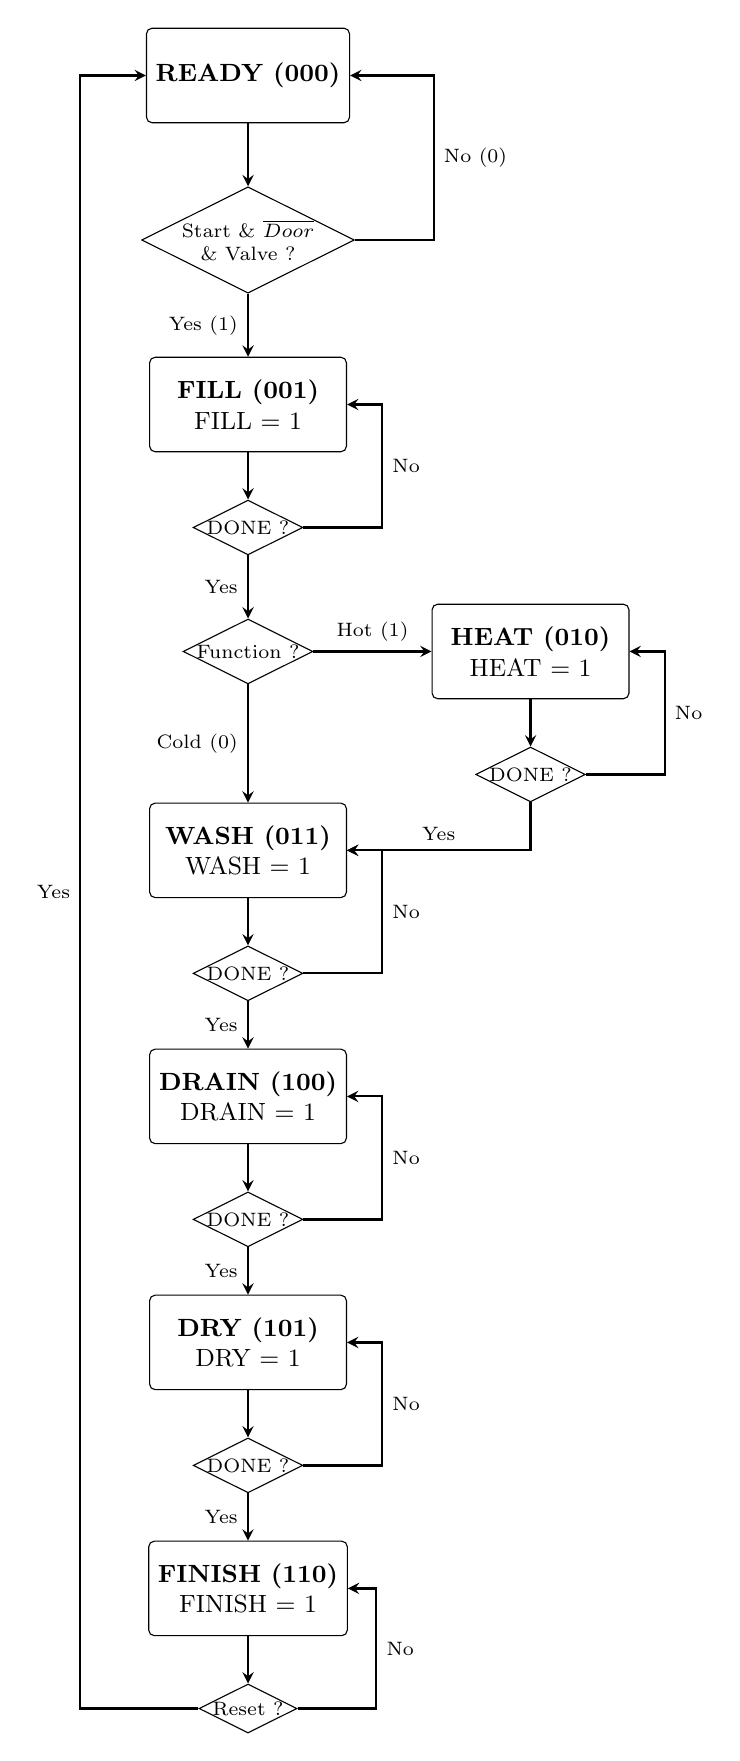
\begin{tikzpicture}[
			node distance=0.6cm and 1.5cm,
			state/.style={rectangle, draw, minimum width=2.5cm, minimum height=1.2cm, text centered, align=center, rounded corners=2pt, font=\small},
			decision/.style={diamond, draw, aspect=2, text centered, align=center, inner sep=0pt, font=\scriptsize},
			arrow/.style={thick, ->, >=stealth},
			font=\sffamily
			]
			
			% Nodes
			\node[state] (ready) {\textbf{READY (000)}};
			\node[decision, below=of ready, yshift=-0.2cm] (start) {Start \& $\overline{Door}$\\\& Valve ?};
			\node[state, below=of start, yshift=-0.2cm] (fill) {\textbf{FILL (001)}\\FILL = 1};
			\node[decision, below=of fill] (done1) {DONE ?};
			\node[decision, below=of done1, yshift=-0.2cm] (func) {Function ?};
			
			\node[state, right=1.5cm of func] (heat) {\textbf{HEAT (010)}\\HEAT = 1};
			\node[decision, below=of heat] (done2) {DONE ?};
			
			\node[state, below=1.5cm of func] (wash) {\textbf{WASH (011)}\\WASH = 1};
			\node[decision, below=of wash] (done3) {DONE ?};
			
			\node[state, below=of done3] (drain) {\textbf{DRAIN (100)}\\DRAIN = 1};
			\node[decision, below=of drain] (done4) {DONE ?};
			
			\node[state, below=of done4] (dry) {\textbf{DRY (101)}\\DRY = 1};
			\node[decision, below=of dry] (done5) {DONE ?};
			
			\node[state, below=of done5] (finish) {\textbf{FINISH (110)}\\FINISH = 1};
			\node[decision, below=of finish] (reset) {Reset ?};
			
			% Arrows
			\draw[arrow] (ready) -- (start);
			\draw[arrow] (start.east) -- ++(1,0) |- node[pos=0.25, right, font=\scriptsize] {No (0)} (ready.east);
			\draw[arrow] (start.south) -- node[left, font=\scriptsize] {Yes (1)} (fill.north);
			
			\draw[arrow] (fill) -- (done1);
			\draw[arrow] (done1.east) -- ++(1,0) |- node[pos=0.25, right, font=\scriptsize] {No} (fill.east);
			\draw[arrow] (done1.south) -- node[left, font=\scriptsize] {Yes} (func.north);
			
			\draw[arrow] (func.east) -- node[above, font=\scriptsize] {Hot (1)} (heat.west);
			\draw[arrow] (func.south) -- node[left, font=\scriptsize] {Cold (0)} (wash.north);
			
			\draw[arrow] (heat) -- (done2);
			\draw[arrow] (done2.east) -- ++(1,0) |- node[pos=0.25, right, font=\scriptsize] {No} (heat.east);
			\draw[arrow] (done2.south) |- node[pos=0.75, above, font=\scriptsize] {Yes} (wash.east);
			
			\draw[arrow] (wash) -- (done3);
			\draw[arrow] (done3.east) -- ++(1,0) |- node[pos=0.25, right, font=\scriptsize] {No} (wash.east);
			\draw[arrow] (done3.south) -- node[left, font=\scriptsize] {Yes} (drain.north);
			
			\draw[arrow] (drain) -- (done4);
			\draw[arrow] (done4.east) -- ++(1,0) |- node[pos=0.25, right, font=\scriptsize] {No} (drain.east);
			\draw[arrow] (done4.south) -- node[left, font=\scriptsize] {Yes} (dry.north);
			
			\draw[arrow] (dry) -- (done5);
			\draw[arrow] (done5.east) -- ++(1,0) |- node[pos=0.25, right, font=\scriptsize] {No} (dry.east);
			\draw[arrow] (done5.south) -- node[left, font=\scriptsize] {Yes} (finish.north);
			
			\draw[arrow] (finish) -- (reset);
			\draw[arrow] (reset.east) -- ++(1,0) |- node[pos=0.25, right, font=\scriptsize] {No} (finish.east);
			\draw[arrow] (reset.west) -- ++(-1.5,0) |- node[pos=0.25, left, font=\scriptsize] {Yes} (ready.west);
			
		\end{tikzpicture}
		\endL
		\caption{نمودار حالت ماشین لباسشویی}
		\label{fig:asm-chart}
	\end{figure}
	
	\subsection{بلوک‌دیاگرام کلی مدار}
	پیش از ورود به جزئیات سیم‌کشی، بلوک‌دیاگرام کلی این مدار در شکل \ref{fig:block-washing} نشان داده شده است. همان‌طور که دیده می‌شود، مدار از سه بخش اصلی تشکیل شده است:
	\begin{enumerate}
		\item \textbf{رجیستر وضعیت و منطق وضعیت بعدی} شامل سه فلیپ‌فلاپ \lr{D} و مداری ترکیبی از گیت‌های \lr{AND/OR} که وظیفه محاسبه وضعیت بعدی ($Q_2^+, Q_1^+, Q_0^+$)  بر عهده دارند.
		\item \textbf{تایمر سنکرون (تراشه 74163):} این شمارنده وظیفه ایجاد تاخیرهای زمانی را دارد.
		\item \textbf{منطق تشخیص اتمام زمان (DONE):} این بخش با بررسی وضعیت فعلی، تشخیص می‌دهد که آیا در یک وضعیت ۲-سیکلی (آب‌گیری، تخلیه، خشک‌کردن) هستیم یا ۳-سیکلی (گرم‌کردن، شست‌وشو). به محض رسیدن تایمر به مقدار مطلوب، سیگنال $DONE$ یک شده و به منطق وضعیت بعدی فرمان عبور می‌دهد.
	\end{enumerate}
	
	\begin{figure}[htbp]
		\centering
		\beginL
		\begin{tikzpicture}[
			node distance=0.8cm and 1.2cm,
			block/.style={rectangle, draw, thick, minimum height=1.1cm, minimum width=2.6cm, align=center, fill=gray!8},
			io/.style={rectangle, draw, thick, minimum height=0.8cm, minimum width=1.6cm, align=center, fill=blue!6},
			sig/.style={-{Latex[length=2mm]}, thick}
			]
			
			\node[io] (inputs) {\RL{ورودی‌ها}\\$Start, Door$\\$Valve, Func$\\$Reset$};
			\node[block, right=of inputs, minimum height=2.5cm] (nsl) {\RL{منطق}\\\RL{وضعیت بعدی}\\(Next State)};
			\node[block, right=of nsl, minimum height=2.5cm] (reg) {\RL{رجیستر وضعیت}\\(3x D-FF)\\$Q_2, Q_1, Q_0$};
			\node[block, right=of reg, minimum height=2.5cm] (outlogic) {\RL{منطق خروجی}\\(Output Logic)};
			\node[io, below=of outlogic] (outputs) {\RL{خروجی‌ها}\\$Fill, Heat$\\$Wash, Drain$\\$Dry, Finish$};
			
			\node[block, below=1.2cm of reg, minimum height=1.5cm] (timer) {\RL{تایمر و منطق}\\$DONE$\\(74163)};
			\node[io, below=0.8cm of timer] (clk) {$Clock$};
			
			\draw[sig] (inputs) -- (nsl);
			\draw[sig] (nsl) -- (reg);
			\draw[sig] (reg) -- (outlogic);
			\draw[sig] (outlogic) -- (outputs);
			\draw[sig] (clk) -- (timer);
			
			% Feedback from reg to nsl
			\draw[sig] (reg.north) -- ++(0,0.6) -| node[pos=0.25, above, font=\scriptsize] {\RL{وضعیت فعلی} \lr{($Q_2, Q_1, Q_0$)}} (nsl.north);
			
			% Reg to Timer
			\draw[sig] (reg) -- node[right, font=\scriptsize] {\RL{وضعیت فعلی}} (timer);
			
			% Timer to NSL
			\draw[sig] (timer.west) -| node[pos=0.25, above, font=\scriptsize] {\RL{سیگنال} $DONE$} (nsl.south);
			
		\end{tikzpicture}
		\endL
		\caption{بلوک‌دیاگرام کلی مدار کنترل‌کننده ماشین لباسشویی}
		\label{fig:block-washing}
	\end{figure}
	
	\subsection{استخراج معادلات منطقی و طراحی مدار}
	برای پیاده‌سازی بلوک منطق وضعیت بعدی (\lr{Next State Logic})، باید رفتار سیستم را در قالب یک جدول گذار حالت توصیف کنیم. ماشین لباسشویی دارای ۷ حالت است که توسط سه فلیپ‌فلاپ $Q_2, Q_1, Q_0$ کدگذاری شده‌اند. 
	
	متغیرهای ورودی موثر در تغییر حالت عبارتند از:
	\begin{itemize}
		\item $S$: فشردن کلید استارت ($Start$)
		\item $D$: بسته بودن در ($Door=0$، در معادلات به‌صورت $\overline{D}$ استفاده می‌شود)
		\item $V$: باز بودن شیر آب ($Valve$)
		\item $F$: انتخاب برنامه شست‌وشو ($Function$؛ ۱ برای آب گرم و ۰ برای آب سرد)
		\item $DN$: اتمام زمان تایمر در هر مرحله ($DONE$)
		\item $R$: فشردن کلید ریست ($Reset$)
	\end{itemize}
	
	جدول زیر شرایط لازم برای رفتن به وضعیت بعدی را نشان می‌دهد. با توجه به این جدول، می‌توان معادلات \lr{SOP} را برای ورودی \lr{D} هر فلیپ‌فلاپ ($Q_2^+, Q_1^+, Q_0^+$) استخراج کرد.
	
	\clearpage
	
	\begin{table}[h]
		\centering
		\resizebox{\textwidth}{!}{
			\begin{LTR}
				\begin{tabular}{|c|c|c|c|p{6cm}|}
					\hline
					\textbf{\rl{حالت فعلی} \lr{($Q_2 Q_1 Q_0$)}} & \textbf{\rl{نام حالت}} & \textbf{\rl{وضعیت بعدی}} & \textbf{\rl{شرط گذار (انتقال)}} & \multicolumn{1}{c|}{\textbf{\textpersian{توضیحات}}} \\ \hline
					\multirow{2}{*}{000} & \multirow{2}{*}{READY} & 001 (FILL) & $S \cdot \overline{D} \cdot V$ & \setRTL \textpersian{با استارت، درِ بسته و شیرِ باز به آب‌گیری می‌رود.} \\ \cline{3-5} 
					& & 000 (READY) & $\overline{S \cdot \overline{D} \cdot V}$ & \setRTL \textpersian{در غیر این صورت در حالت آماده می‌ماند.} \\ \hline
					
					\multirow{3}{*}{001} & \multirow{3}{*}{FILL} & 010 (HEAT) & $DN \cdot F$ & \setRTL \textpersian{اگر تایمر تمام شود و برنامه آب گرم باشد.} \\ \cline{3-5} 
					& & 011 (WASH) & $DN \cdot \overline{F}$ & \setRTL \textpersian{اگر تایمر تمام شود و برنامه آب سرد باشد.} \\ \cline{3-5} 
					& & 001 (FILL) & $\overline{DN}$ & \setRTL \textpersian{تا اتمام تایمر در آب‌گیری می‌ماند.} \\ \hline
					
					\multirow{2}{*}{010} & \multirow{2}{*}{HEAT} & 011 (WASH) & $DN$ & \setRTL \textpersian{پس از اتمام گرم‌کردن به شست‌وشو می‌رود.} \\ \cline{3-5} 
					& & 010 (HEAT) & $\overline{DN}$ & \setRTL \textpersian{تا اتمام تایمر در گرم‌کردن می‌ماند.} \\ \hline
					
					\multirow{2}{*}{011} & \multirow{2}{*}{WASH} & 100 (DRAIN) & $DN$ & \setRTL \textpersian{پس از اتمام شست‌وشو به تخلیه می‌رود.} \\ \cline{3-5} 
					& & 011 (WASH) & $\overline{DN}$ & \setRTL \textpersian{تا اتمام تایمر در شست‌وشو می‌ماند.} \\ \hline
					
					\multirow{2}{*}{100} & \multirow{2}{*}{DRAIN} & 101 (DRY) & $DN$ & \setRTL \textpersian{پس از اتمام تخلیه به خشک‌کردن می‌رود.} \\ \cline{3-5} 
					& & 100 (DRAIN) & $\overline{DN}$ & \setRTL \textpersian{تا اتمام تایمر در تخلیه می‌ماند.} \\ \hline
					
					\multirow{2}{*}{101} & \multirow{2}{*}{DRY} & 110 (FINISH) & $DN$ & \setRTL \textpersian{پس از اتمام خشک‌کردن به پایان می‌رود.} \\ \cline{3-5} 
					& & 101 (DRY) & $\overline{DN}$ & \setRTL \textpersian{تا اتمام تایمر در خشک‌کردن می‌ماند.} \\ \hline
					
					\multirow{2}{*}{110} & \multirow{2}{*}{FINISH} & 000 (READY) & $R$ & \setRTL \textpersian{با فشردن ریست به حالت آماده برمی‌گردد.} \\ \cline{3-5} 
					& & 110 (FINISH) & $\overline{R}$ & \setRTL \textpersian{در غیر این صورت در پایان قفل می‌شود.} \\ \hline
				\end{tabular}
			\end{LTR}
		}
		\caption{جدول گذار حالت برای ماشین لباسشویی}
		\label{tab:state-transition-washing}
	\end{table}
	
	با استخراج معادلات از جدول بالا، باید تمام شرایطی که باعث یک‌شدن هر فلیپ‌فلاپ در وضعیت بعدی می‌شوند را با یکدیگر \lr{OR} کنیم. معادلات نهایی (به‌فرم \lr{SOP}) به شکل زیر به‌دست می‌آیند:
	
	\paragraph{معادلهٔ فلیپ‌فلاپ $Q_0$ (LSB):}
	این بیت در وضعیت‌های \lr{FILL (001)}، \lr{WASH (011)} و \lr{DRY (101)} یک است.
	\begin{align*}
		Q_0^+ = \;& (READY \cdot S \cdot \overline{D} \cdot V) + (FILL \cdot \overline{DN}) + (FILL \cdot DN \cdot \overline{F}) \\
		&+ (HEAT \cdot DN) + (WASH \cdot \overline{DN}) + (DRAIN \cdot DN) + (DRY \cdot \overline{DN})
	\end{align*}
	
	\paragraph{معادلهٔ فلیپ‌فلاپ $Q_1$:}
	این بیت در وضعیت‌های \lr{HEAT (010)}، \lr{WASH (011)} و \lr{FINISH (110)} یک است.
	\begin{align*}
		Q_1^+ = \;& (FILL \cdot DN \cdot F) + (HEAT \cdot \overline{DN}) + (FILL \cdot DN \cdot \overline{F}) \\
		&+ (HEAT \cdot DN) + (WASH \cdot \overline{DN}) + (DRY \cdot DN) + (FINISH \cdot \overline{R})
	\end{align*}
	
	\paragraph{معادلهٔ فلیپ‌فلاپ $Q_2$ (MSB):}
	این بیت در وضعیت‌های \lr{DRAIN (100)}، \lr{DRY (101)} و \lr{FINISH (110)} یک است.
	\begin{align*}
		Q_2^+ = \;& (WASH \cdot DN) + (DRAIN \cdot \overline{DN}) + (DRAIN \cdot DN) \\
		&+ (DRY \cdot \overline{DN})+ (DRY \cdot DN) + (FINISH \cdot \overline{R})
	\end{align*}
	
	\subsection{طراحی در پروتئوس}
	در این بخش، پیاده‌سازی مدار در محیط پروتئوس انجام شده است. برای ساخت ماشین حالت از سه فلیپ‌فلاپ \lr{74LS74} استفاده کردیم. از آنجا که طراحی بر اساس معادلات \lr{SOP} انجام شده است، خروجی‌های گیت‌های \lr{AND} مربوط به هر مسیرِ گذار، در نهایت وارد گیت‌های \lr{OR} چندورودی ($Q_0^+, Q_1^+, Q_2^+$) شده و به ورودی \lr{D} فلیپ‌فلاپ‌ها متصل شده‌اند. 
	
	تایمر مدار با استفاده از تراشه \lr{74163} بسته شده است. گیت \lr{NOR} متصل به پایه \lr{CLR} این تراشه تضمین می‌کند که با هر بار تغییر وضعیت (یک شدن سیگنال $DONE$)، تایمر به صورت سنکرون صفر شود تا زمان‌سنجی مرحله بعدی کاملاً دقیق انجام گیرد.
	
	در شکل \ref{fig:proteus-washing} شماتیک نهایی مدار پیاده‌سازی شده در پروتئوس قابل مشاهده است.
	
	در شکل~\ref{fig:proteus-washing} نمای کلی شماتیک آمده است. نماهای نزدیک بلوک‌ها به‌صورت جداگانه در شکل‌های~\ref{fig:wash-in} تا~\ref{fig:wash-ns} (ورودی‌ها، خروجی‌ها، رجیستر وضعیت، تایمر و منطق ترکیبی وضعیت بعدی) دیده می‌شوند.
	
	\clearpage
	
	\begin{figure}[htbp]
		\centering
		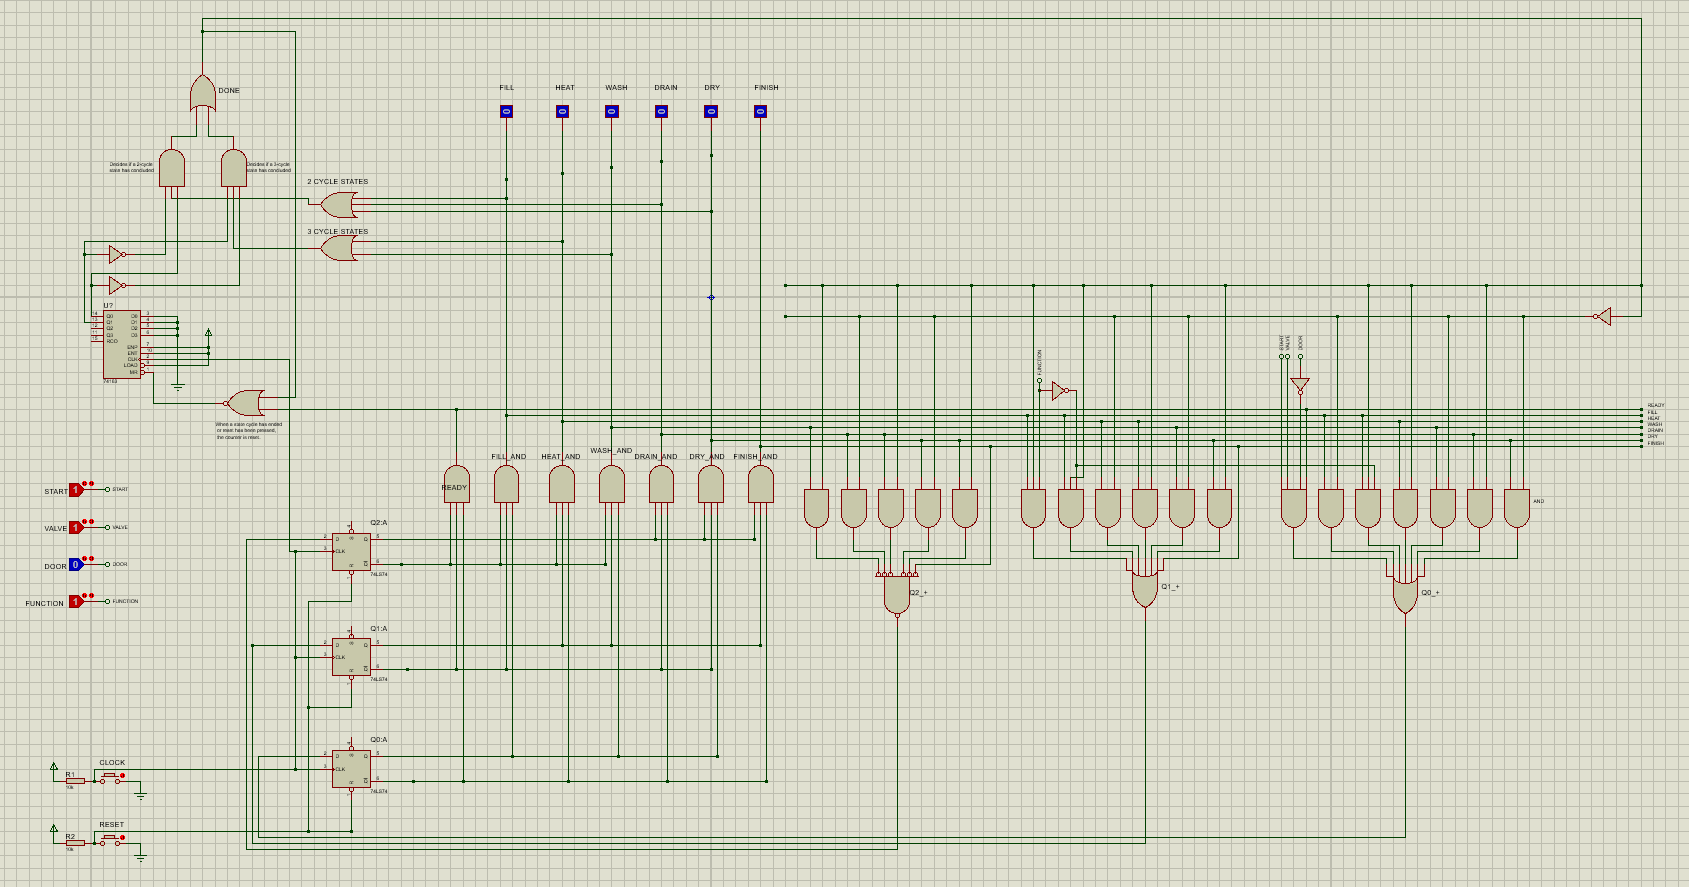
\includegraphics[width=\textwidth]{fig_4_1_1.png}
		\caption{نمای کلی پیاده‌سازی مدار کنترل‌کننده ماشین لباسشویی در محیط پروتئوس}
		\label{fig:proteus-washing}
	\end{figure}
	
	\begin{figure}[htbp]
		\centering
		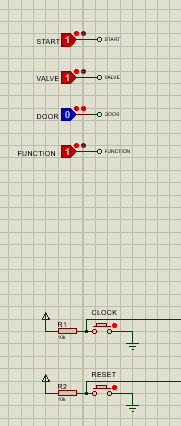
\includegraphics[width=0.28\textwidth]{fig_4_1_2.png}
		\caption{نگاه نزدیک به سیگنال‌های ورودی مدار لباسشویی}
		\label{fig:wash-in}
	\end{figure}
	
	\begin{figure}[htbp]
		\centering
		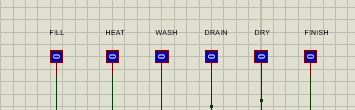
\includegraphics[width=0.70\textwidth]{fig_4_1_3.png}
		\caption{نگاه نزدیک به سیگنال‌های خروجی مدار لباسشویی}
		\label{fig:wash-out}
	\end{figure}
	
	\begin{figure}[htbp]
		\centering
		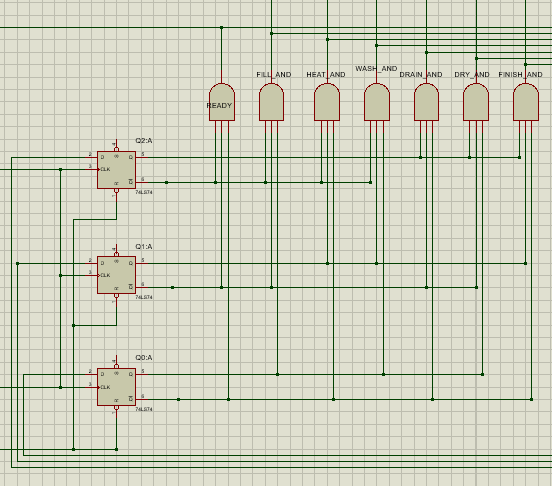
\includegraphics[width=0.62\textwidth]{fig_4_1_4.png}
		\caption{نگاه نزدیک به رجیستر وضعیت مدار لباسشویی}
		\label{fig:wash-reg}
	\end{figure}
	
	\begin{figure}[htbp]
		\centering
		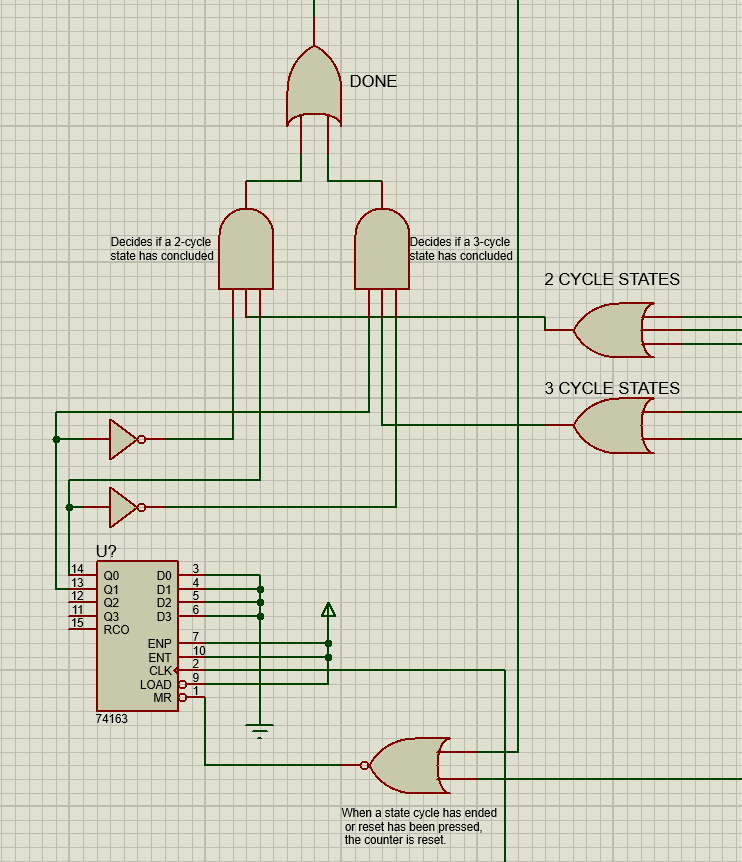
\includegraphics[width=0.58\textwidth]{fig_4_1_6.png}
		\caption{نگاه نزدیک به تایمر \lr{74163} مدار لباسشویی}
		\label{fig:wash-timer}
	\end{figure}
	
	\begin{figure}[htbp]
		\centering
		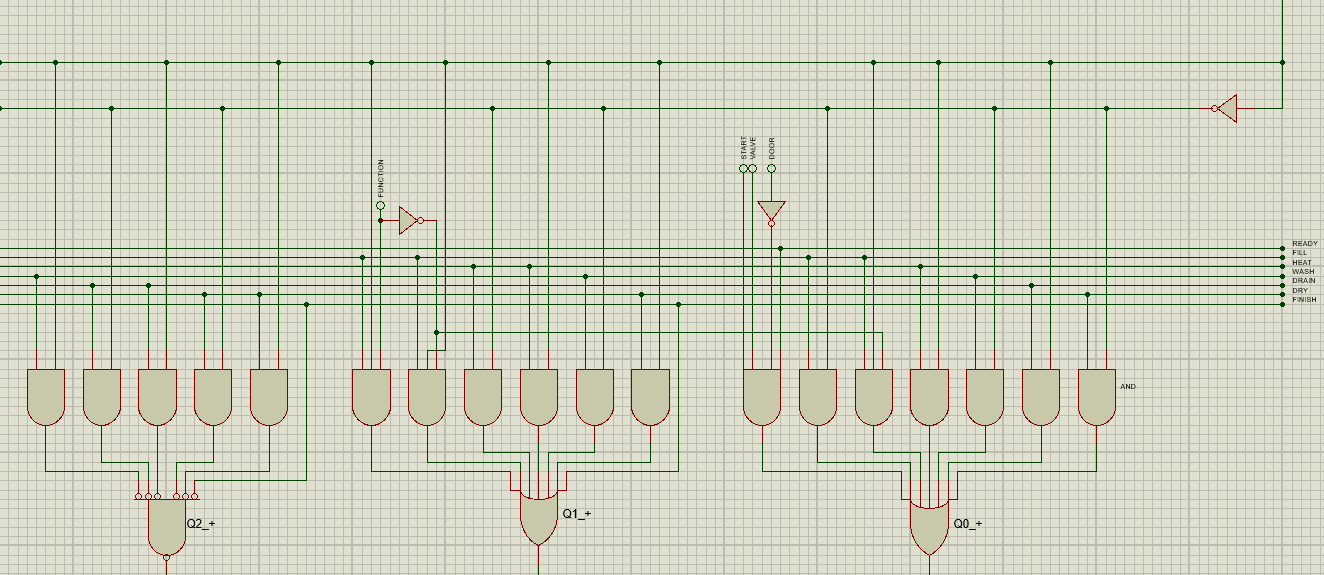
\includegraphics[width=\textwidth]{fig_4_1_5.png}
		\caption{نگاه نزدیک به مدار ترکیبی تولید وضعیت بعدی لباسشویی}
		\label{fig:wash-ns}
	\end{figure}
	
	\clearpage
	
	\subsection{بررسی Test Case ها}
	در طول آزمایش، صحت عملکرد مدار با اعمال سناریوهای مختلف بررسی شد. مهم‌ترین این سناریوها عبارتند از:
	\begin{itemize}
		\item \textbf{شست‌وشو با آب سرد ($Function=0$):} با فشردن کلید $Start$ در حالی که در و شیر آب بسته‌اند، مدار وارد حالت $FILL$ شده و پس از ۲ پالس کلاک، مستقیماً به حالت $WASH$ پرش می‌کند (حالت $HEAT$ نادیده گرفته می‌شود). شرایط شروع این سناریو در شکل~\ref{fig:wash-cold-start} و خروجی‌های گام‌به‌گام در $t=0,2,5,7,9$ در شکل~\ref{fig:wash-cold-seq} آمده است.
		\item \textbf{شست‌وشو با آب گرم ($Function=1$):} با اعمال این ورودی، مدار پس از $FILL$ وارد حالت $HEAT$ شده و دقیقاً پس از ۳ پالس کلاک، وارد مرحله $WASH$ می‌شود. شرایط شروع و خروجی در $t=2$ در شکل~\ref{fig:wash-hot} دیده می‌شود. از آنجا که مرحلهٔ $HEAT$ سه کلاک طول می‌کشد، خروجی کلاک‌های بعدی این سناریو با همان شکل‌های مسیر آب سرد، با شیفت زمانی ۳ کلاک، قابل تطبیق است ($t=5,8,10,12$ آب گرم متناظر با $t=2,5,7,9$ آب سرد).
		\item \textbf{بررسی زمان‌بندی‌ها:} با مشاهده گام‌به‌گام کلاک‌ها، اطمینان حاصل شد که وضعیت‌های ۲-سیکلی و ۳-سیکلی دقیقاً در زمان مقرر سیگنال $DONE$ را تولید کرده و به وضعیت بعدی شیفت می‌کنند.
	\end{itemize}
	
	\clearpage
	
	\begin{figure}[htbp]
		\centering
		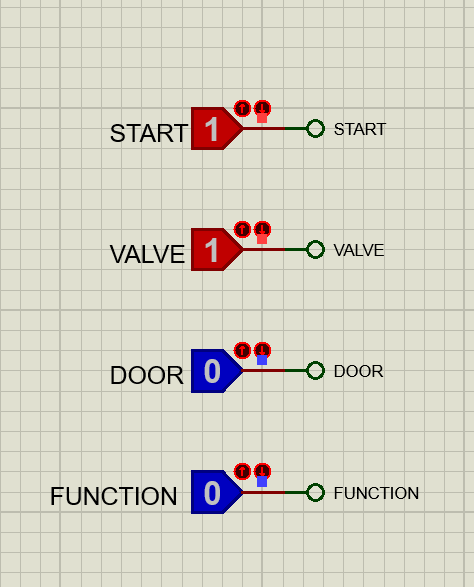
\includegraphics[width=0.55\textwidth]{fig_4_1_7.png}
		\caption{شرایط شروع تست‌کیس شست‌وشو با آب سرد}
		\label{fig:wash-cold-start}
	\end{figure}
	
	\begin{figure}[htbp]
		\centering
		\begin{subfigure}[b]{0.48\textwidth}
			\centering
			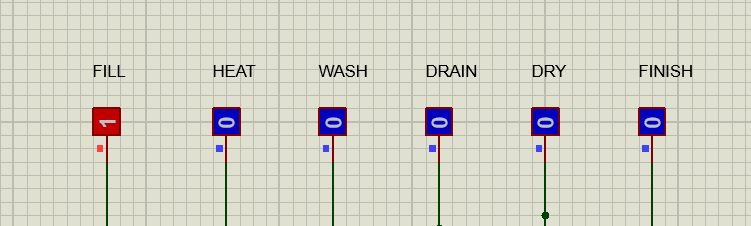
\includegraphics[width=\textwidth]{fig_4_1_8.png}
			\caption{$t=0$}
			\label{fig:wash-t0}
		\end{subfigure}
		\hfill
		\begin{subfigure}[b]{0.48\textwidth}
			\centering
			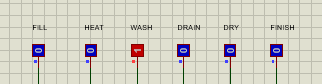
\includegraphics[width=\textwidth]{fig_4_1_9.png}
			\caption{$t=2$}
			\label{fig:wash-t2}
		\end{subfigure}
		
		\vspace{1em}
		
		\begin{subfigure}[b]{0.48\textwidth}
			\centering
			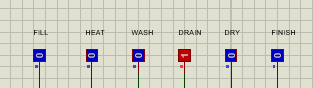
\includegraphics[width=\textwidth]{fig_4_1_10.png}
			\caption{$t=5$}
			\label{fig:wash-t5}
		\end{subfigure}
		\hfill
		\begin{subfigure}[b]{0.48\textwidth}
			\centering
			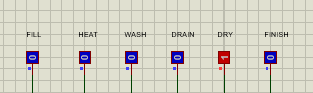
\includegraphics[width=\textwidth]{fig_4_1_11.png}
			\caption{$t=7$}
			\label{fig:wash-t7}
		\end{subfigure}
		
		\vspace{1em}
		
		\begin{subfigure}[b]{0.48\textwidth}
			\centering
			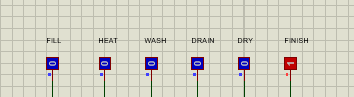
\includegraphics[width=\textwidth]{fig_4_1_12.png}
			\caption{$t=9$}
			\label{fig:wash-t9}
		\end{subfigure}
		\caption{خروجی مدار لباسشویی در مسیر آب سرد در کلاک‌های متوالی}
		\label{fig:wash-cold-seq}
	\end{figure}
	
	\begin{figure}[htbp]
		\centering
		\begin{subfigure}[b]{0.32\textwidth}
			\centering
			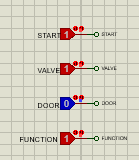
\includegraphics[width=\textwidth]{fig_4_1_13.png}
			\caption{شروع مسیر آب گرم}
			\label{fig:wash-hot-start}
		\end{subfigure}
		\hfill
		\begin{subfigure}[b]{0.64\textwidth}
			\centering
			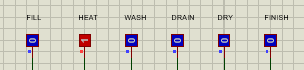
\includegraphics[width=\textwidth]{fig_4_1_14.png}
			\caption{خروجی در $t=2$ مسیر آب گرم}
			\label{fig:wash-hot-t2}
		\end{subfigure}
		\caption{تست‌کیس شست‌وشو با آب گرم؛ کلاک‌های بعدی همان توالی شکل~\ref{fig:wash-cold-seq} با سه واحد تأخیر زمانی است}
		\label{fig:wash-hot}
	\end{figure}
	
	\clearpage
	
	% ---------- Section 4 ----------
	\section{طراحی و ساخت مدار کنترل‌کننده تلفن راه‌دور}
	
	\subsection{طراحی و رسم نمودار حالت}
	در این بخش، مدار کنترل‌کننده یک تلفن راه‌دور طراحی شده است. پیش از پیاده‌سازی، رفتار سیستم را با استفاده از\lr{ASM Chart} مدل‌سازی می‌کنیم. این مدار دارای ۴ وضعیت اصلی است که برای کدگذاری آن‌ها به ۲ فلیپ‌فلاپ ($Q_1, Q_0$) نیاز داریم:
	
	\begin{itemize}
		\item \textbf{READY (00):} دستگاه آماده است. منتظر فشردن کلید $Start$ و وجود حداقل یک سکه ($COINS>0$) در دستگاه است.
		\item \textbf{CALL (01):} تماس برقرار است. در این حالت سیگنال $CALL$ فعال است و با هر بار اتمام تایمر $T_1$ یک سکه کسر می‌شود.
		\item \textbf{ALARM (11):} موجودی سکه‌ها صفر شده است. سیگنال‌های $CALL$ و $ALARM$ هر دو فعال هستند. مدار منتظر ورود سکه جدید یا اتمام مهلت $T_2$ است.
		\item \textbf{IDLE\_ALARM (10):} مهلت $T_2$ تمام شده و تماسی قطع شده است، اما سیگنال $ALARM$ همچنان روشن است (قفل هشدار). تنها با ورود سکه جدید می‌توان از این حالت خارج شد.
	\end{itemize}
	
	
	\begin{figure}[htbp]
		\centering
		\beginL
		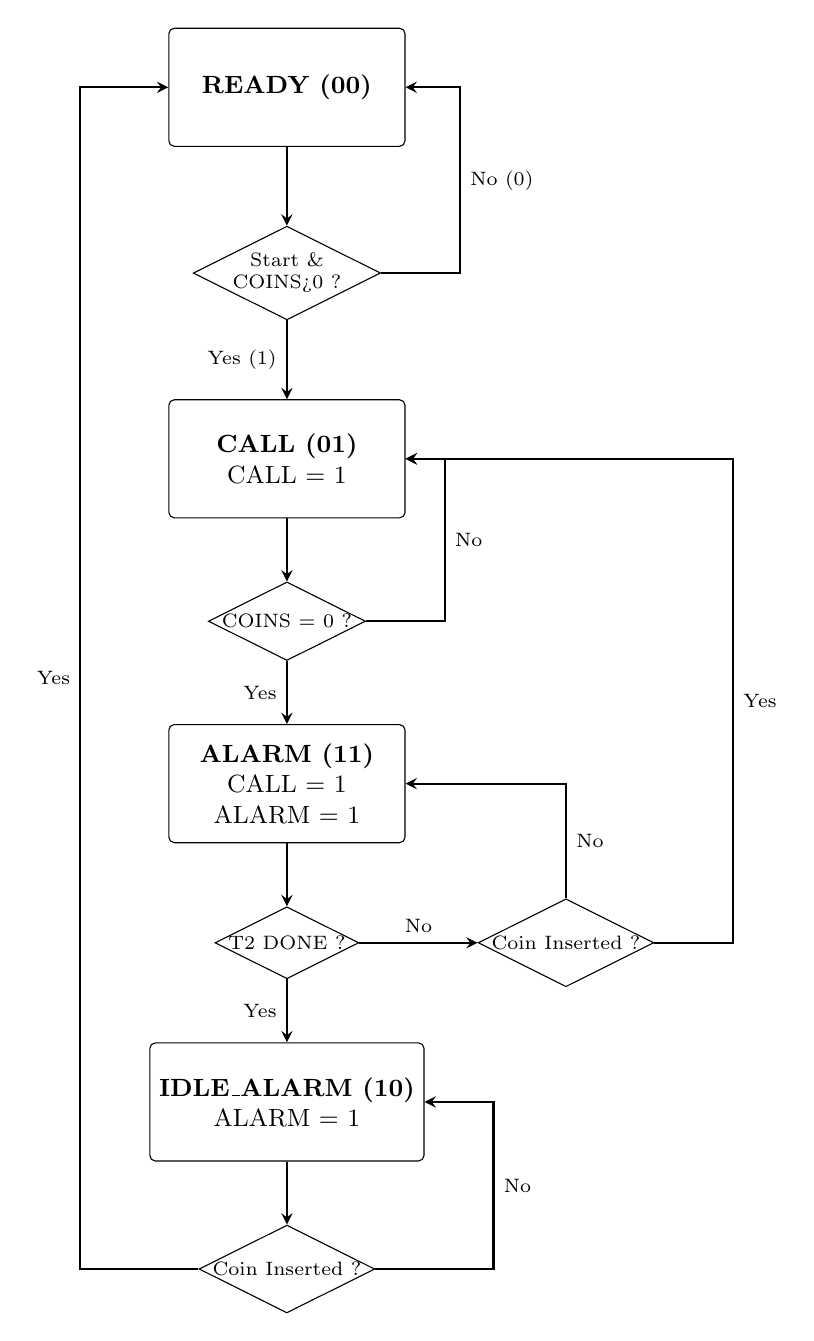
\begin{tikzpicture}[
			node distance=0.8cm and 1.5cm,
			state/.style={rectangle, draw, minimum width=3cm, minimum height=1.5cm, text centered, align=center, rounded corners=2pt, font=\small},
			decision/.style={diamond, draw, aspect=2, text centered, align=center, inner sep=0pt, font=\scriptsize},
			arrow/.style={thick, ->, >=stealth},
			font=\sffamily
			]
			
			% Nodes
			\node[state] (ready) {\textbf{READY (00)}};
			\node[decision, below=of ready, yshift=-0.2cm] (start) {Start \&\\COINS>0 ?};
			
			\node[state, below=of start, yshift=-0.2cm] (call) {\textbf{CALL (01)}\\CALL = 1};
			
			\node[decision, below=of call] (coins0) {COINS = 0 ?};
			
			\node[state, below=of coins0] (alarm) {\textbf{ALARM (11)}\\CALL = 1\\ALARM = 1};
			
			\node[decision, below=of alarm] (t2done) {T2 DONE ?};
			\node[decision, right=1.5cm of t2done] (coin_inserted1) {Coin Inserted ?};
			
			\node[state, below=of t2done] (idle) {\textbf{IDLE\_ALARM (10)}\\ALARM = 1};
			
			\node[decision, below=of idle] (coin_inserted2) {Coin Inserted ?};
			
			% Arrows
			\draw[arrow] (ready) -- (start);
			\draw[arrow] (start.east) -- ++(1,0) |- node[pos=0.25, right, font=\scriptsize] {No (0)} (ready.east);
			\draw[arrow] (start.south) -- node[left, font=\scriptsize] {Yes (1)} (call.north);
			
			\draw[arrow] (call) -- (coins0);
			\draw[arrow] (coins0.east) -- ++(1,0) |- node[pos=0.25, right, font=\scriptsize] {No} (call.east);
			\draw[arrow] (coins0.south) -- node[left, font=\scriptsize] {Yes} (alarm.north);
			
			\draw[arrow] (alarm) -- (t2done);
			\draw[arrow] (t2done.east) -- (coin_inserted1.west) node[midway, above, font=\scriptsize] {No};
			
			% Routing for Coin Inserted (during ALARM)
			\draw[arrow] (coin_inserted1.north) |- node[pos=0.25, right, font=\scriptsize] {No} (alarm.east);
			\draw[arrow] (coin_inserted1.east) -- ++(1,0) |- node[pos=0.25, right, font=\scriptsize] {Yes} (call.east);
			
			\draw[arrow] (t2done.south) -- node[left, font=\scriptsize] {Yes} (idle.north);
			
			\draw[arrow] (idle) -- (coin_inserted2);
			\draw[arrow] (coin_inserted2.east) -- ++(1.5,0) |- node[pos=0.25, right, font=\scriptsize] {No} (idle.east);
			\draw[arrow] (coin_inserted2.west) -- ++(-1.5,0) |- node[pos=0.25, left, font=\scriptsize] {Yes} (ready.west);
			
		\end{tikzpicture}
		\endL
		\caption{نمودار حالت تلفن راه‌دور}
		\label{fig:asm-chart-telephone}
	\end{figure}
	
	\subsection{بلوک‌دیاگرام کلی مدار}
	بلوک‌دیاگرام کلی مدار تلفن راه‌دور در شکل \ref{fig:block-telephone} نشان داده شده است. این مدار از سه بخش اصلی تشکیل شده است:
	\begin{enumerate}
		\item \textbf{رجیستر وضعیت:} شامل ۲ فلیپ‌فلاپ \lr{D} و شبکه‌ای از گیت‌های \lr{AND/OR} که وظیفه محاسبه وضعیت بعدی ($Q_1^+, Q_0^+$) را بر عهده دارند.
		\item \textbf{شمارنده سکه‌ها (\lr{Coin Counter}):} شامل دو تراشه \lr{74192} (شمارنده \lr{BCD}) که تعداد سکه‌ها را ذخیره می‌کند. .
		\item \textbf{تایمر سنکرون:} تراشه \lr{74163} که زمان‌های $T_1$ (برای کسر دوره‌ای سکه) و $T_2$ (مهلت قطع تماس) را اندازه‌گیری می‌کند.
	\end{enumerate}
	
	\begin{figure}[htbp]
		\centering
		\beginL
		\begin{tikzpicture}[
			node distance=1.5cm and 2cm,
			block/.style={rectangle, draw, thick, minimum height=1.1cm, minimum width=2.6cm, align=center, fill=gray!8},
			io/.style={rectangle, draw, thick, minimum height=0.8cm, minimum width=1.6cm, align=center, fill=blue!6},
			sig/.style={-{Latex[length=2mm]}, thick}
			]
			
			\node[io] (inputs) {\RL{ورودی‌ها}\\$Start$\\$Reset$};
			\node[block, right=of inputs, minimum height=2.5cm] (nsl) {\RL{منطق}\\\RL{وضعیت بعدی}\\(Next State)};
			\node[block, right=of nsl, minimum height=2.5cm] (reg) {\RL{رجیستر وضعیت}\\(2x D-FF)\\$Q_1, Q_0$};
			\node[io, right=of reg] (outputs) {\RL{خروجی‌ها}\\$Call, Alarm$};
			
			\node[block, below=1.5cm of reg, minimum height=1.5cm] (timer) {\RL{تایمر}\\(74163)};
			\node[block, below=1.5cm of nsl, minimum height=1.5cm] (counter) {\RL{شمارنده سکه}\\\lr{(2x 74192)}};
			
			\node[io, below=1cm of counter] (coin) {$Coin$ \RL{(کلید)}};
			\node[io, below=1cm of timer] (clk) {$Clock$};
			
			\draw[sig] (inputs) -- (nsl);
			\draw[sig] (nsl) -- (reg);
			\draw[sig] (reg) -- (outputs);
			
			\draw[sig] (clk) -- (timer);
			\draw[sig] (clk) -- (coin);
			\draw[sig] (coin) -- (counter);
			
			% Feedback from reg to nsl (Top)
			\draw[sig] (reg.north) -- ++(0,0.8) -| node[pos=0.25, above, font=\scriptsize] {\RL{وضعیت فعلی} \lr{{($Q_1, Q_0$)}}} (nsl.north);
			
			% Reg to Timer
			\draw[sig] (reg) -- node[right, font=\scriptsize] {\RL{وضعیت}} (timer);
			
			% Timer to Counter
			\draw[sig] (timer.west) -- node[above, font=\scriptsize] {$T_1, T_2$} (counter.east);
			
			% Counter to NSL
			\draw[sig] (counter.north) -- node[left, font=\scriptsize, align=right] {$COINS$} (nsl.south);
			
		\end{tikzpicture}
		\endL
		\caption{بلوک‌دیاگرام کلی مدار کنترل‌کننده تلفن راه‌دور}
		\label{fig:block-telephone}
	\end{figure}
	
	\clearpage
	
	\subsection{استخراج معادلات منطقی و طراحی مدار}
	برای پیاده‌سازی بلوک منطق وضعیت بعدی (\lr{Next State Logic})، رفتار سیستم را در قالب یک جدول درستی می‌نویسیم. متغیرهای ورودی موثر در تغییر حالت عبارتند از:
	\begin{itemize}
		\item $S$: فشردن کلید استارت ($Start$)
		\item $C$: وجود سکه در دستگاه ($COINS>0$)
		\item $\overline{C}$: اتمام سکه‌ها ($COINS=0$)
		\item $T_2$: اتمام زمان تایمر دوم
	\end{itemize}
	
	\begin{table}[htbp]
		\centering
		\resizebox{\textwidth}{!}{
			\begin{LTR}
				\begin{tabular}{|c|c|c|c|p{8cm}|}
					\hline
					\textbf{\rl{حالت فعلی} \lr{($Q_1 Q_0$)}} & \textbf{\rl{نام حالت}} & \textbf{شرط $Q_1^+ = 1$} & \textbf{شرط $Q_0^+ = 1$} & \multicolumn{1}{c|}{\textbf{\textpersian{توضیحات}}} \\ \hline
					00 & READY & 0 & $S \cdot C$ & \setRTL \textpersian{با استارت و وجود سکه به CALL (01) می‌رود.} \\ \hline
					01 & CALL & $\overline{C}$ & $C$ & \setRTL \textpersian{تا وقتی سکه هست در CALL می‌ماند؛ با اتمام سکه به ALARM (11) می‌رود.} \\ \hline
					11 & ALARM & $\overline{C}$ & $C + \overline{T_2}$ & \setRTL \textpersian{تا وقتی سکه نیست در هشدار می‌ماند؛ اگر $T_2$ تمام شود و سکه نباشد به 10 می‌رود.} \\ \hline
					10 & IDLE\_ALARM & $\overline{C}$ & 0 & \setRTL \textpersian{هشدار تا زمانی که سکه ($C$) وارد نشود روشن می‌ماند.} \\ \hline
				\end{tabular}
			\end{LTR}
		}
		\caption{جدول گذار حالت برای فلیپ‌فلاپ‌های $Q_1$ و $Q_0$ در مدار تلفن}
		\label{tab:state-transition-telephone}
	\end{table}
	
	با استفاده از جدول بالا، معادلات منطقی برای ورودی \lr{D} هر فلیپ‌فلاپ (\lr{SOP}) به‌دست می‌آید. 
	
	\paragraph{معادلهٔ فلیپ‌فلاپ $Q_0$:}
	$$Q_0^+ = (READY \cdot S \cdot C) + (CALL \cdot C) + (ALARM \cdot (C + \overline{T_2}))$$
	$$Q_0^+ = (\overline{Q_1}\overline{Q_0} \cdot S \cdot C) + (\overline{Q_1}Q_0 \cdot C) + (Q_1 Q_0 \cdot (C + \overline{T_2}))$$
	
	\paragraph{معادلهٔ فلیپ‌فلاپ $Q_1$:}
	$$Q_1^+ = (CALL \cdot \overline{C}) + (ALARM \cdot \overline{C}) + (IDLE\_ALARM \cdot \overline{C})$$
	$$Q_1^+ = (\overline{Q_1}Q_0 \cdot \overline{C}) + (Q_1 Q_0 \cdot \overline{C}) + (Q_1\overline{Q_0} \cdot \overline{C})$$
	
	\subsection{طراحی در پروتئوس}
	در این بخش، پیاده‌سازی مدار در محیط پروتئوس انجام شده است. یکی از چالش‌های اساسی در این مدار، همگام‌سازی ورودی ناهمگام (کلید فیزیکی سکه) با کلاک سیستم بود. برای جلوگیری از ایجاد گلیچ و کسر اشتباه سکه‌ها، از تکنیک کلاک‌گیتینگ (\lr{Clock Gating}) با ترکیب گیت‌های \lr{NOR} و \lr{OR} استفاده شد تا کسر سکه دقیقاً در لبهٔ بالاروندهٔ کلاک انجام شود. همچنین برای جلوگیری از سرریز شمارنده به ۹۹ در زمان اتمام سکه‌ها، یک مدار تشخیص صفر (\lr{0-Guard}) با گیت \lr{NAND} تعبیه شد که پالس کسر سکه را در حالت $COINS=0$ مسدود می‌کند.
	
	در شکل \ref{fig:proteus-telephone} شماتیک نهایی مدار پیاده‌سازی شده در پروتئوس قابل مشاهده است.
	
	در شکل~\ref{fig:proteus-telephone} نمای کلی شماتیک آمده است. نماهای نزدیک بلوک‌ها به‌صورت جداگانه در شکل‌های~\ref{fig:tel-in} تا~\ref{fig:tel-ns} (ورودی‌ها و منطق کسر سکه، نمایشگر سکه، تایمر، رجیستر وضعیت و منطق تعیین وضعیت بعدی) دیده می‌شوند.
	
	\begin{figure}[htbp]
		\centering
		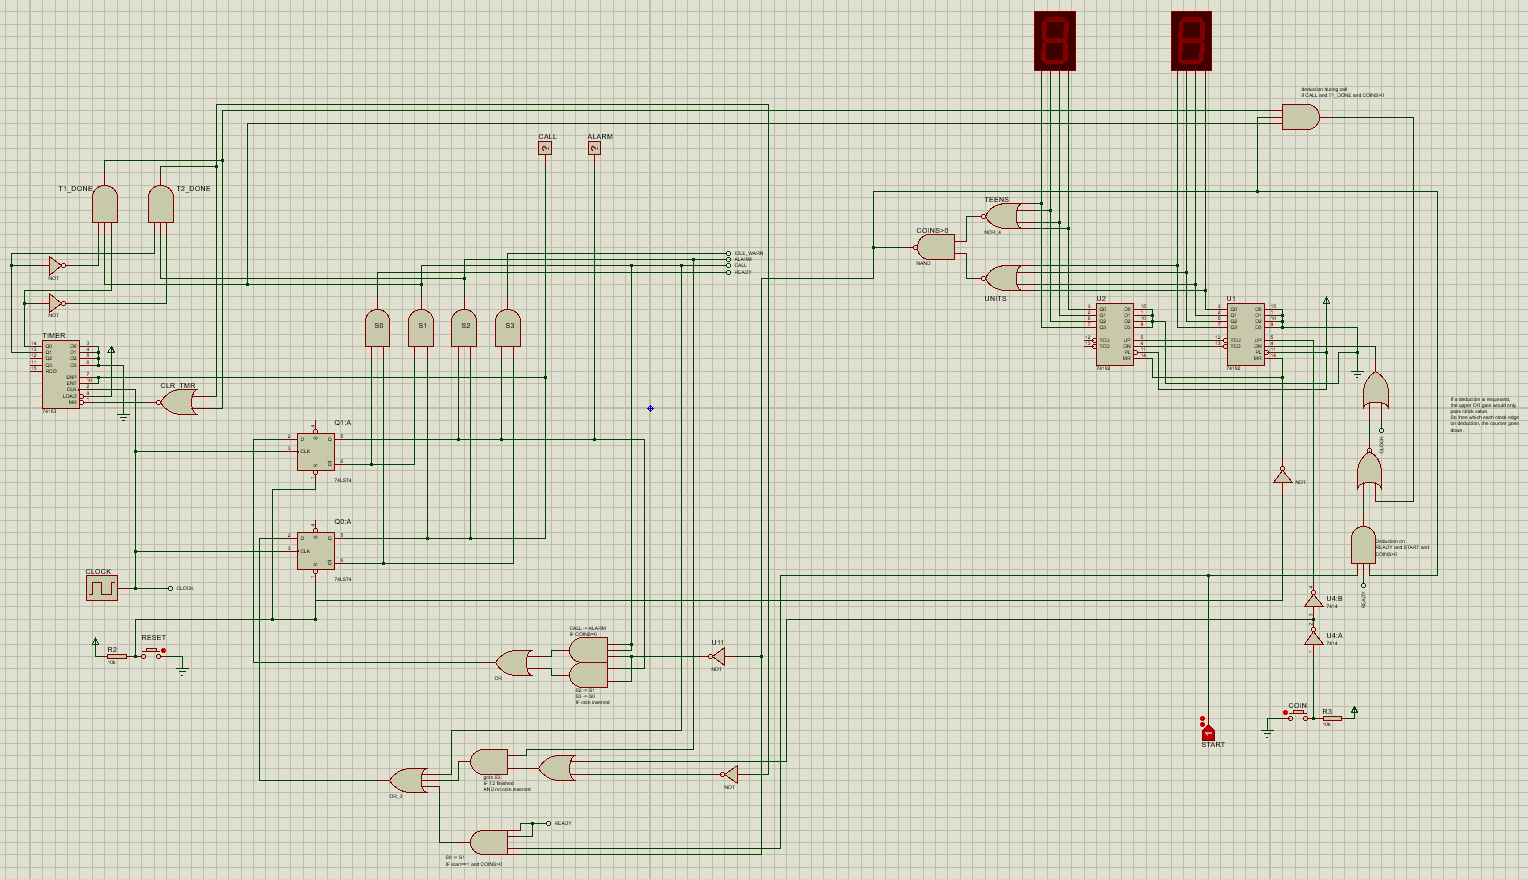
\includegraphics[width=\textwidth]{fig_4_2_1.png}
		\caption{نمای کلی پیاده‌سازی مدار کنترل‌کننده تلفن راه‌دور در محیط پروتئوس}
		\label{fig:proteus-telephone}
	\end{figure}
	
	\begin{figure}[htbp]
		\centering
		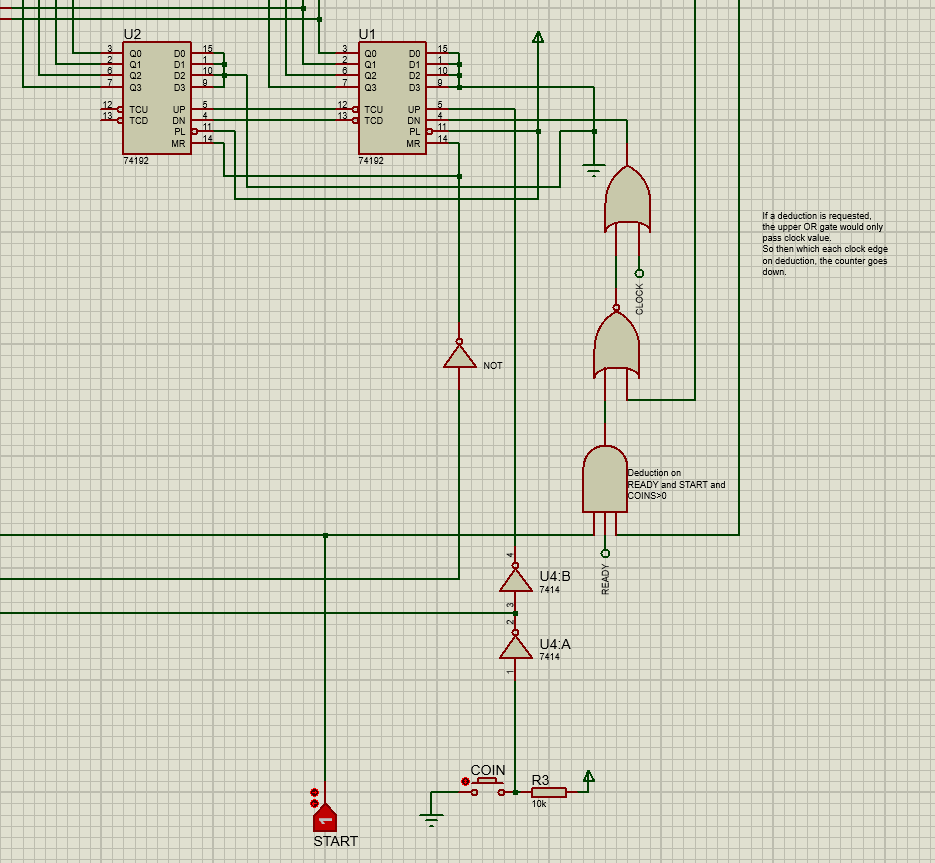
\includegraphics[width=0.78\textwidth]{fig_4_2_2.png}
		\caption{نگاه نزدیک به سیگنال‌های ورودی و منطق کسر سکه}
		\label{fig:tel-in}
	\end{figure}
	
	\begin{figure}[htbp]
		\centering
		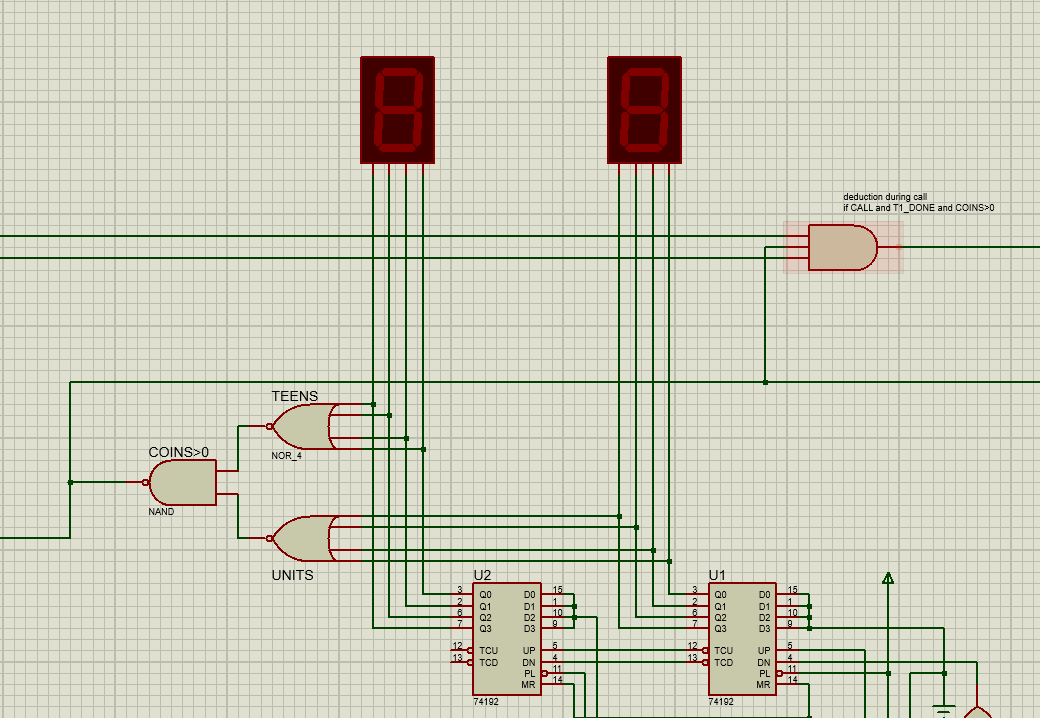
\includegraphics[width=0.82\textwidth]{fig_4_2_3.png}
		\caption{نگاه نزدیک به نمایشگرهای سکه}
		\label{fig:tel-disp}
	\end{figure}
	
	\begin{figure}[htbp]
		\centering
		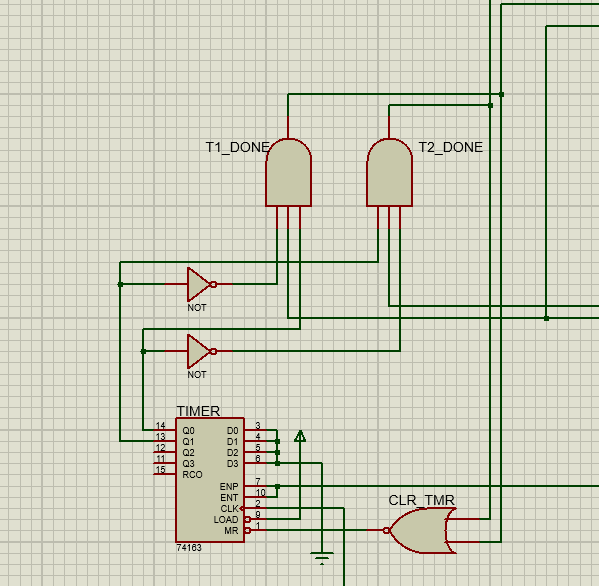
\includegraphics[width=0.62\textwidth]{fig_4_2_4.png}
		\caption{نگاه نزدیک به تایمر مدار تلفن}
		\label{fig:tel-timer}
	\end{figure}
	
	\begin{figure}[htbp]
		\centering
		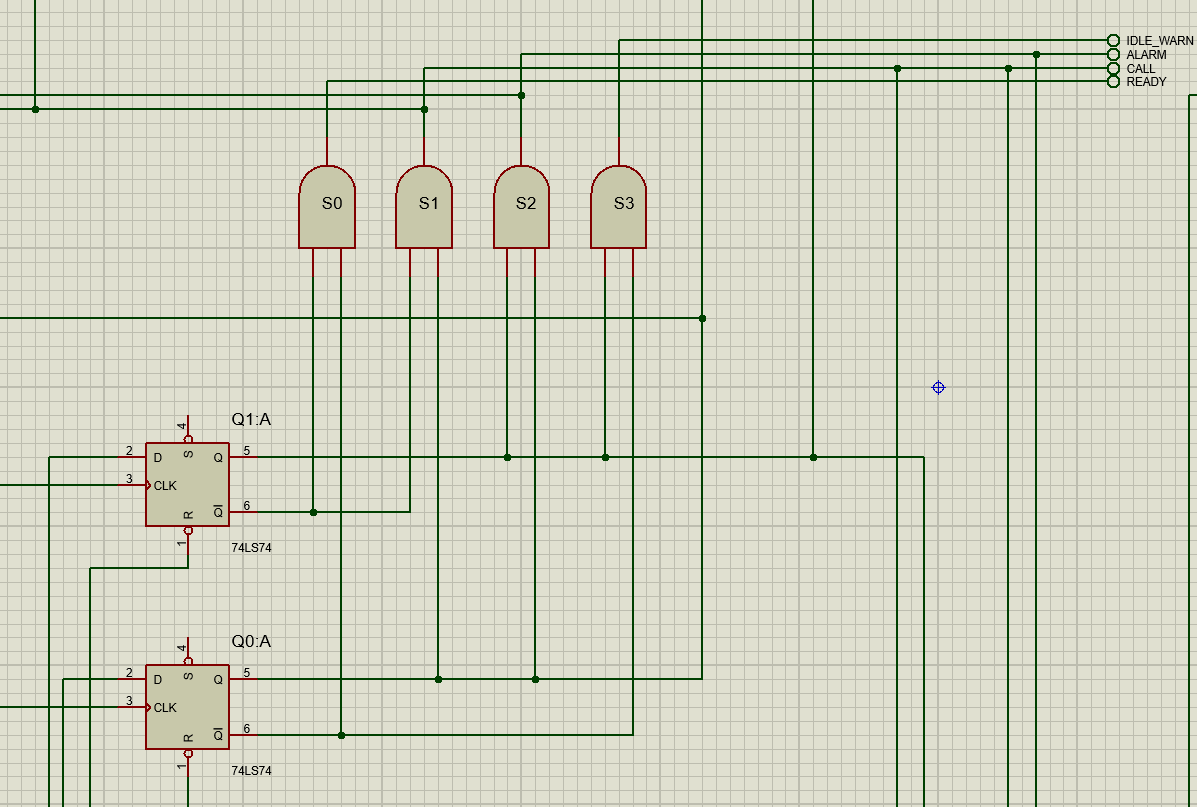
\includegraphics[width=0.88\textwidth]{fig_4_2_5.png}
		\caption{نگاه نزدیک به رجیستر وضعیت مدار تلفن}
		\label{fig:tel-reg}
	\end{figure}
	
	\begin{figure}[htbp]
		\centering
		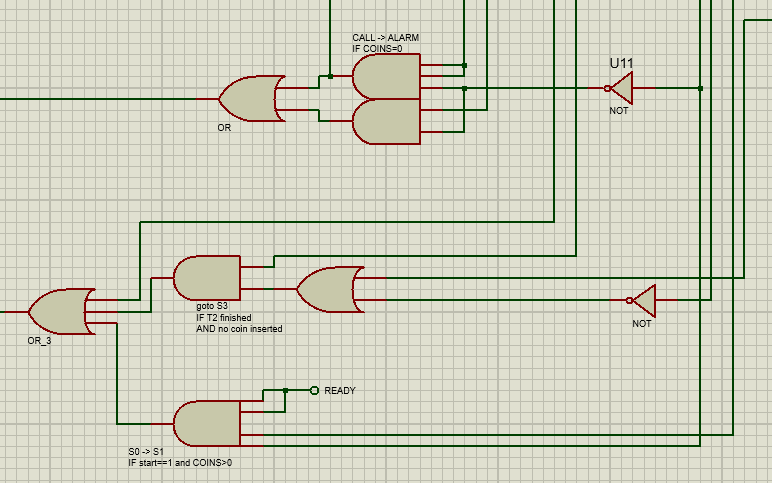
\includegraphics[width=0.80\textwidth]{fig_4_2_6.png}
		\caption{نگاه نزدیک به منطق تعیین وضعیت بعدی مدار تلفن}
		\label{fig:tel-ns}
	\end{figure}
	
	\subsection{بررسی Test Case ها}
	در طول آزمایش، صحت عملکرد مدار تلفن با اعمال سناریوهای مختلف بررسی شد. مهم‌ترین این سناریوها عبارتند از:
	\begin{itemize}
		\item \textbf{شروع تماس و کسر سکه:} با وارد کردن سکه و فشردن کلید $Start$، مدار وارد حالت $CALL$ شده و با هر بار اتمام تایمر $T_1$، یک واحد از شمارنده‌های \lr{BCD} کسر می‌شود. افزایش موجودی تا ۳ سکه در شکل~\ref{fig:tel-coins3} و گذار به $CALL$ همراه با کسر سکه در $t=0$ در شکل~\ref{fig:tel-t0} دیده می‌شود. وضعیت مدار در $t=2$ هنوز در $CALL$ است (شکل~\ref{fig:tel-t2}).
		\item \textbf{اتمام موجودی و هشدار:} به محض رسیدن شمارنده به صفر، مدار بلافاصله وارد حالت $ALARM$ شده و چراغ هشدار روشن می‌شود. در شکل~\ref{fig:tel-t5-alarm} پس از اتمام یک دورهٔ $T_1$ در $t=5$، شرط $\overline{C}$ برقرار شده و در کلاک بعد وضعیت از $CALL$ به $ALARM$ می‌رود.\footnote{گذار $CALL\to ALARM$ روی همان لبه‌ای که آخرین سکه کسر می‌شود رخ نمی‌دهد. شمارندهٔ \lr{BCD} روی لبهٔ بالارونده صفر می‌شود و سیگنال $C=(COINS>0)$ پس از این لبه $\overline{C}$ می‌گردد؛ ماشین مور وضعیت را فقط از روی مقدار ثبت‌شده در فلیپ‌فلاپ‌ها عوض می‌کند، بنابراین $Q_1$ یک کلاک بعد یک می‌شود. این تأخیر یک‌کلاکی با سطر $CALL$ در جدول~\ref{tab:state-transition-telephone} و معادلهٔ $Q_1^+ = CALL\cdot\overline{C}+\cdots$ سازگار است.}
		\item \textbf{تایم‌اوت $T_2$ و قفل هشدار:} اگر در حالت هشدار، سکه‌ای وارد نشود و تایمر $T_2$ به پایان برسد، سیگنال تماس قطع شده اما هشدار روشن می‌ماند (حالت $IDLE\_ALARM$). این مسیر در $t=7$ در شکل~\ref{fig:tel-t7-idle} آمده است.
		\item \textbf{بازیابی تماس:} با وارد کردن سکه در حین حالت هشدار، مدار فوراً از حالت $ALARM$ خارج شده و تماس را از سر می‌گیرد. ورود سکه در همان لحظهٔ $t=5$ در شکل~\ref{fig:tel-t5-coin} این مسیر را نشان می‌دهد.
	\end{itemize}
	
	\clearpage
	
	\begin{figure}[htbp]
		\centering
		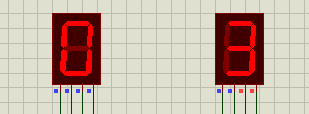
\includegraphics[width=0.55\textwidth]{fig_4_2_7.png}
		\caption{تست‌کیس افزایش موجودی تا ۳ سکه}
		\label{fig:tel-coins3}
	\end{figure}
	
	\begin{figure}[htbp]
		\centering
		\begin{subfigure}[b]{0.48\textwidth}
			\centering
			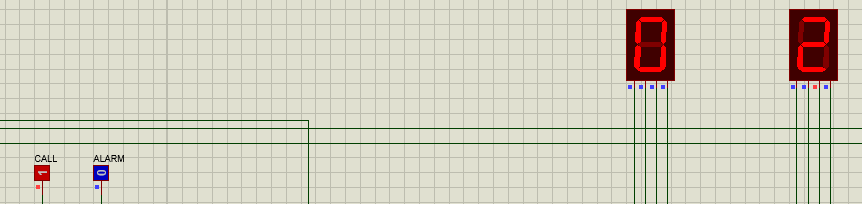
\includegraphics[width=\textwidth]{fig_4_2_8.png}
			\caption{کسر سکه و ورود به $CALL$ در $t=0$}
			\label{fig:tel-t0}
		\end{subfigure}
		\hfill
		\begin{subfigure}[b]{0.48\textwidth}
			\centering
			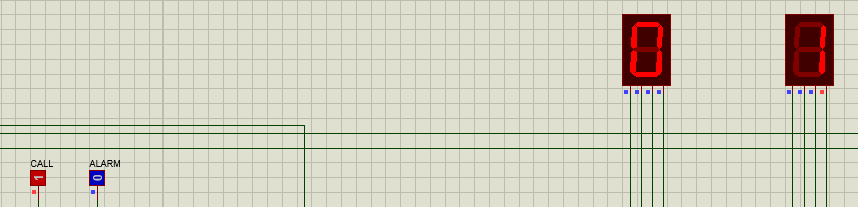
\includegraphics[width=\textwidth]{fig_4_2_9.png}
			\caption{مدار در $t=2$ (همچنان $CALL$)}
			\label{fig:tel-t2}
		\end{subfigure}
		
		\vspace{1em}
		
		\begin{subfigure}[b]{0.48\textwidth}
			\centering
			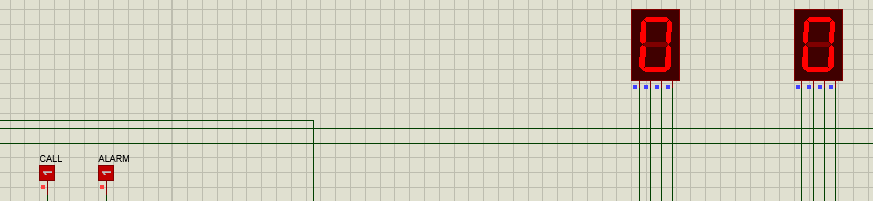
\includegraphics[width=\textwidth]{fig_4_2_10.png}
			\caption{$t=5$ پس از یک $T_1$؛ گذار $CALL$ به $ALARM$ در کلاک بعد}
			\label{fig:tel-t5-alarm}
		\end{subfigure}
		\hfill
		\begin{subfigure}[b]{0.48\textwidth}
			\centering
			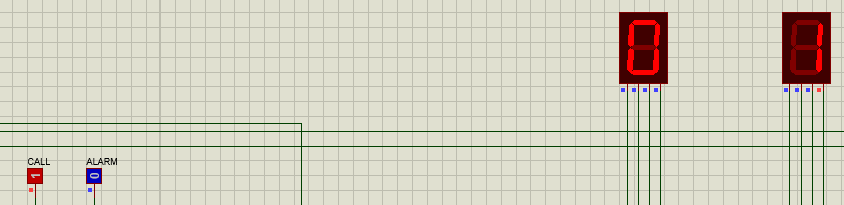
\includegraphics[width=\textwidth]{fig_4_2_14.png}
			\caption{$t=5$ در صورت ورود سکه (بازیابی تماس)}
			\label{fig:tel-t5-coin}
		\end{subfigure}
		
		\vspace{1em}
		
		\begin{subfigure}[b]{0.70\textwidth}
			\centering
			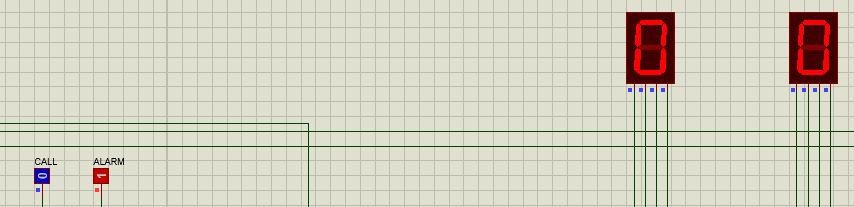
\includegraphics[width=\textwidth]{fig_4_2_13.png}
			\caption{$t=7$ اگر سکه‌ای وارد نشود (مسیر $IDLE\_ALARM$)}
			\label{fig:tel-t7-idle}
		\end{subfigure}
		\caption{نمایش قدم‌به‌قدم عملکرد مدار تلفن در حالت‌های تماس، هشدار، تایم‌اوت و بازیابی}
		\label{fig:test-cases-telephone}
	\end{figure}
	
	\clearpage
	
	% ---------- Section 5 ----------
	\section{نتیجه‌گیری}
	
	در این آزمایش با اصول طراحی و پیاده‌سازی مدارهای کنترل‌کننده (ماشین‌های حالت) بر اساس حالات انتزاعی سیستم و نمودار حالت (\lr{ASM Chart}) آشنا شدیم. برخلاف آزمایش‌های قبلی که تمرکز بر روی بلوک‌های مجزا (مانند شیفت‌رجیسترها یا شمارنده‌ها) بود، در این آزمایش دیدیم که چطور هسته و بلوک کنترل کننده حالت در کنار باقی اجزا مدار قرار می‌گیرد و با آنها ارتباط دارد.
	
	در پیاده‌سازی \textbf{مدار ماشین لباسشویی}، نحوهٔ مدیریت وضعیت‌های متوالی با تاخیرهای زمانی متفاوت را بررسی کردیم. استفاده از تایمر \lr{74163} و تولید سیگنال \lr{DONE} به ما نشان داد که چگونه می‌توان زمان‌بندی مراحل مختلف (مانند آب‌گیری، شست‌وشو و خشک‌کردن) را بدون نیاز به افزایش تعداد فلیپ‌فلاپ‌های وضعیت، به‌صورت سنکرون و دقیق کنترل کرد. همچنین با استفاده از متغیرهای ورودی (مانند انتخاب آب گرم یا سرد)، مسیرهای گذار متفاوتی را در ماشین حالت پیاده‌سازی کردیم.
	
	در طراحی \textbf{مدار تلفن راه‌دور}، با چالش‌های پیچیده‌تری در زمینهٔ همگام‌سازی سیگنال‌های آسنکرون روبرو شدیم. از آنجا که ورود سکه توسط کاربر (فشردن کلید فیزیکی) کاملاً مستقل از کلاک سیستم رخ می‌دهد، اتصال مستقیم آن به شمارنده‌های حساس می‌توانست منجر به ایجاد گلیچ و خطا شود. برای حل این مشکل، از تکنیک کلاک‌گیتینگ (\lr{Clock Gating}) و مدارهای محافظتی (مانند \lr{0-Guard}) استفاده کردیم تا کسر سکه دقیقاً در لبهٔ بالاروندهٔ کلاک سیستم و تنها در صورت وجود موجودی معتبر انجام شود. همچنین با طراحی یک ماشین مور (\lr{Moore})، توانستیم خروجی‌های هشدار و تماس را به‌صورت پایدار و بدون نوسان تولید کنیم.
	
	به‌طور کلی، این آزمایش اهمیت تبدیل وضعیت های انتزاعی یک سیستم به جداول گذار حالت، استخراج معادلات منطقی بهینه و در نهایت، پیاده‌سازی عملی آن یک FSM را در مدارهای دیجیتال را به‌خوبی نشان داد.
	
	
\end{document}